\documentclass{beamer}
\usetheme{metropolis}
\usepackage{graphicx}
\usepackage{amsmath}
\usepackage{tcolorbox}
\title{College Writing Seminar (INTD100): Week 2 Notes}
\author{Jordan Hanson}
\institute{Whittier College Department of Physics and Astronomy}

\begin{document}
\maketitle

\section{Summary}

\begin{frame}{Summary}
\textbf{Week 2}: \textit{Concise writing II:} In Week 2, we will focus on reading a piece of science writing, and creating your \textit{own} writing that tailors the story to a particular audience.
\begin{itemize}
\item Exercises: work in teams to produce a piece of science writing intended for a broad audience that weaves together information from a variety of sources: (a) a TED talk (b) a scientific journal article (c) and resources like Wikipedia and Google Scholar
\item Homework: writing a post designed for social media about a piece of science that grabs the attention of a wide audience, and attempts to convince that audience that the science is interesting
\item Exploration topic: Black hole observations
\end{itemize}
\end{frame}

\section{Group Project}

\begin{frame}{Group Project: Collaborative Science Writing}
\textbf{\alert{Instructions}}: Systematically random groups (next slide)
\begin{enumerate}
\item Choose one of the following four topics on the following slides
\item Choose a \textit{corresponding author} who will create a Google Document and share it with the others
\item Select a number of sources pertaining to the topic
\begin{itemize}
\item TED talks
\item Scientific journals from \url{arXiv.org} and \url{scholar.google.com}
\item Sources located on Wikipedia
\end{itemize}
\item Create a map or outline with Coggle.it or other tool that summarizes recent discoveries
\item Write a 1 page, single-spaced, 12 point font summary ($\approx 800-1000$ words)'
\item \alert{Bonus points: including a separate bibliography, correctly formatted}
\end{enumerate}
\end{frame}

\begin{frame}{Group Project: Collaborative Science Writing}
\small
\begin{columns}[T]
\begin{column}{0.5\textwidth}
\begin{enumerate}
\item Grace	Cooper ... Group A
\item Zack	Duhala ... Group B
\item Juan	Estrada ... Group C
\item Jusraunaq	Farmahan ... Group D
\item Mateo	Gomez ... Group A
\item Elise	Hansen ... Group B
\item Wyatt	Killien ... Group C
\item Kyle	Miller ... Group D
\end{enumerate}
\end{column}
\begin{column}{0.5\textwidth}
\begin{enumerate}
\item Eliot	Moser ... Group A
\item Rudy	Reyes ... Group B
\item Nick	Reynolds ... Group C
\item Paulina Valdez ... Group D
\item Andrea Wainwright ... Group A
\item Natasha Waldorf ... Group B
\item Emma Walston ... Group C
\end{enumerate}
\end{column}
\end{columns}
\end{frame}

\begin{frame}{Group Project: Collaborative Science Writing}
\small
\underline{Science Topics}
\begin{enumerate}
\item Event Horizon Telescope and the First Picture of a Black Hole
\begin{itemize}
\item What is long-baseline interferometry?
\item What are the properties of the black hole observed?
\end{itemize}
\item LIGO, Virgo and the First Neutron Star - Black Hole Merger
\begin{itemize}
\item What is a neutron star?
\item What is a black hole neutron stare merger?
\end{itemize}
\item IceCube Neutrino Observatory
\begin{itemize}
\item What is a neutrino?
\item What is IceCube Neutrino Observatory and where is it located?
\item What major discoveries have they made so far?
\end{itemize}
\item Anything related to COVID-19 and the pandemic
\begin{itemize}
\item How is the rate of spread quantified?
\item How fatal is the virus, and how does this vary for people?
\end{itemize}
\end{enumerate}
\end{frame}

\begin{frame}{Group Project: Collaborative Science Writing}
\small
\underline{Source classes}
\begin{enumerate}
\item TED talks: surprisingly useful at the start: \url{https://www.ted.com/talks/katie_bouman_how_to_take_a_picture_of_a_black_hole?utm_campaign=tedspread&utm_medium=referral&utm_source=tedcomshare}
\item Wikipedia has more sources: Event Horizon Telescope \url{https://en.wikipedia.org/wiki/Event_Horizon_Telescope}, references section leads you to \url{arXiv.org} with the exact set of references to journals
\item \url{arXiv.org} and \url{scholar.google.com}, as previously discussed, leads to journals
\item NewScientist, Space.com, Scientific American, etc.
\end{enumerate}
\end{frame}

\begin{frame}{Group Project: Collaborative Science Writing}
\begin{figure}
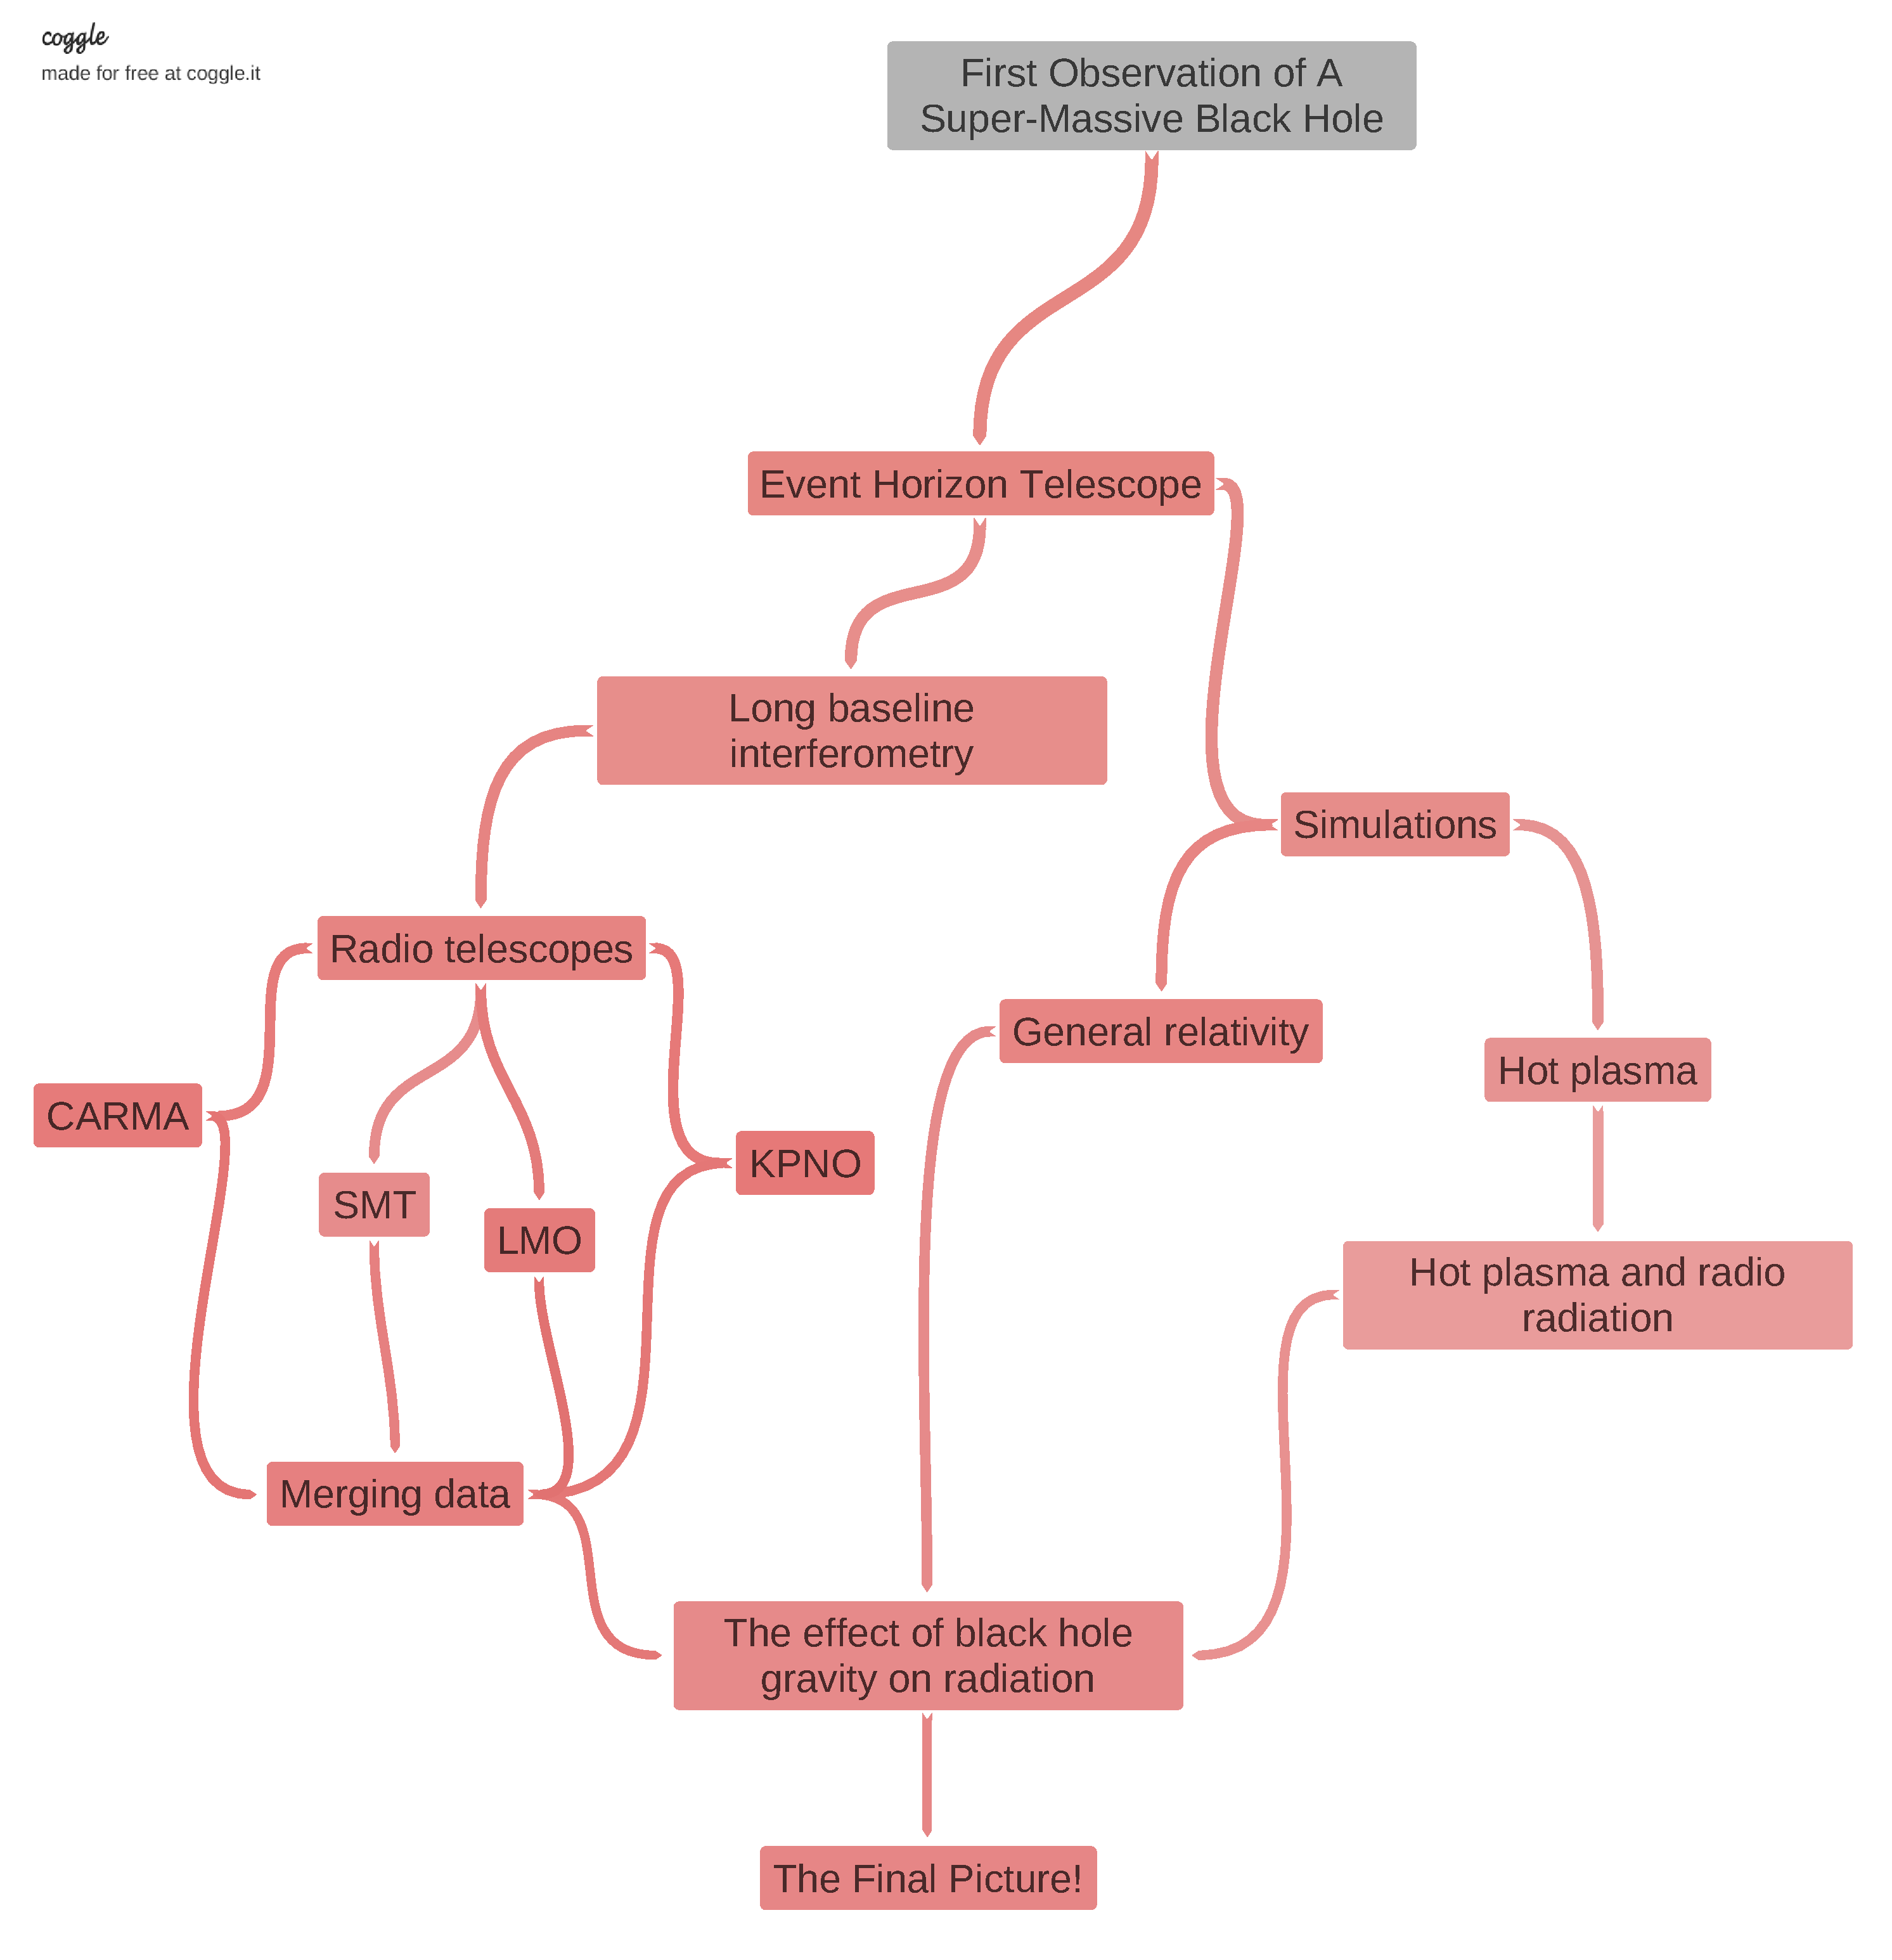
\includegraphics[width=0.65\textwidth]{figures/blackhole.pdf}
\caption{\label{fig:black} Black hole observations and Event Horizon Telescope.}
\end{figure}
\end{frame}

\begin{frame}{Group Project: Collaborative Science Writing}
\underline{Sources to Outline: Which details to cut?}
\begin{enumerate}
\item Kill your darlings
\item Hierarchy of detail: which \textit{level} of detail to cut?
\item Using analogies to replace finest details, equations
\item Cite or quote experts where appropriate
\end{enumerate}
\end{frame}

\begin{frame}{Group Project: Collaborative Science Writing}
\begin{figure}
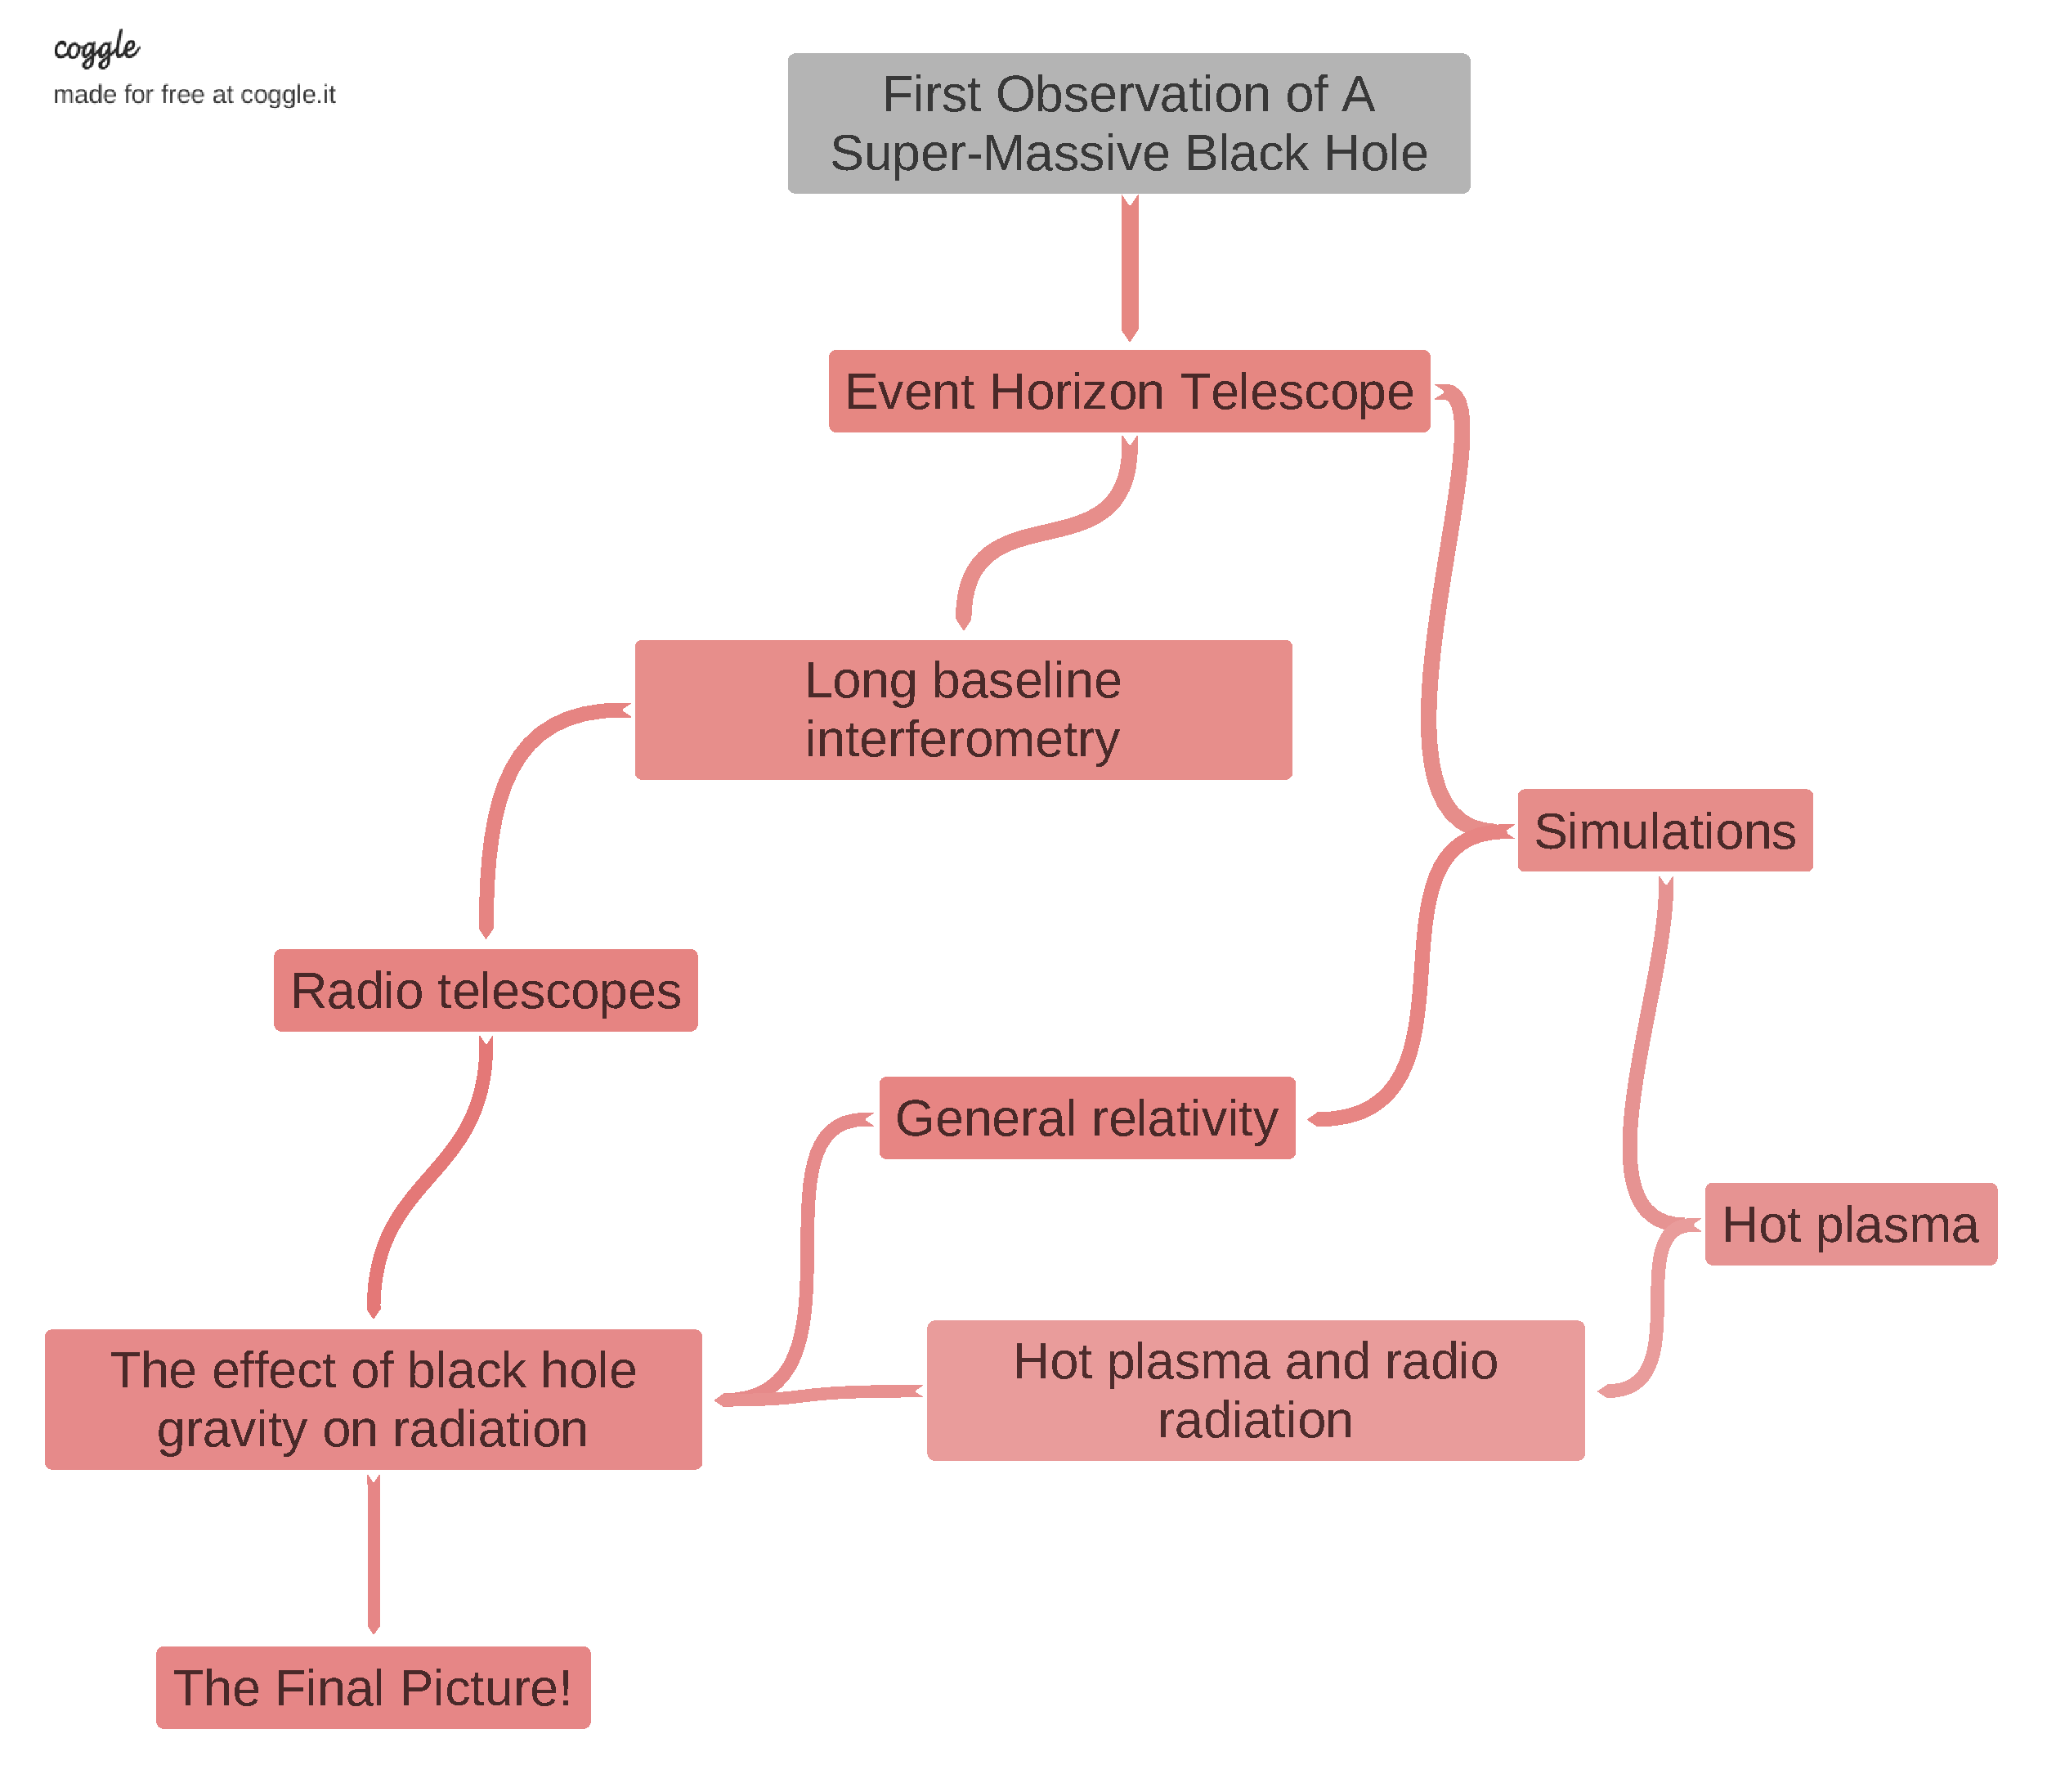
\includegraphics[width=0.65\textwidth]{figures/blackhole2.pdf}
\caption{\label{fig:black2} Black hole observations and Event Horizon Telescope, take 2.}
\end{figure}
\end{frame}

\section{Example: COVID-19 for a General Audience}

\begin{frame}{COVID-19 for a General Audience}
Review of general steps:
\begin{itemize}
\item Build a small list of sources
\item Create a map or outline
\item Write for each bubble or branch
\item Edit and polish the finished tract
\end{itemize}
\end{frame}

\begin{frame}{COVID-19 for a General Audience}
\alert{How do you ... \textit{start} ... building a set of sources?}  The first one is a \textit{general article} (written very well, sourced by a credible expert) for a general audience with links to technical work.
\begin{enumerate}
\item ``5 things scientists know about COVID-19 - and 5 they're still figuring out.'' Karen Frances Eng for \url{ideas.ted.com}
\item ``Tracking the Cornonavirus in California.'' LA Times
\item \url{https://coronavirus.jhu.edu/map.html}
\item \url{https://ourworldindata.org/coronavirus-data-explorer}
\end{enumerate}
\end{frame}

\begin{frame}{COVID-19 for a General Audience}
\begin{figure}
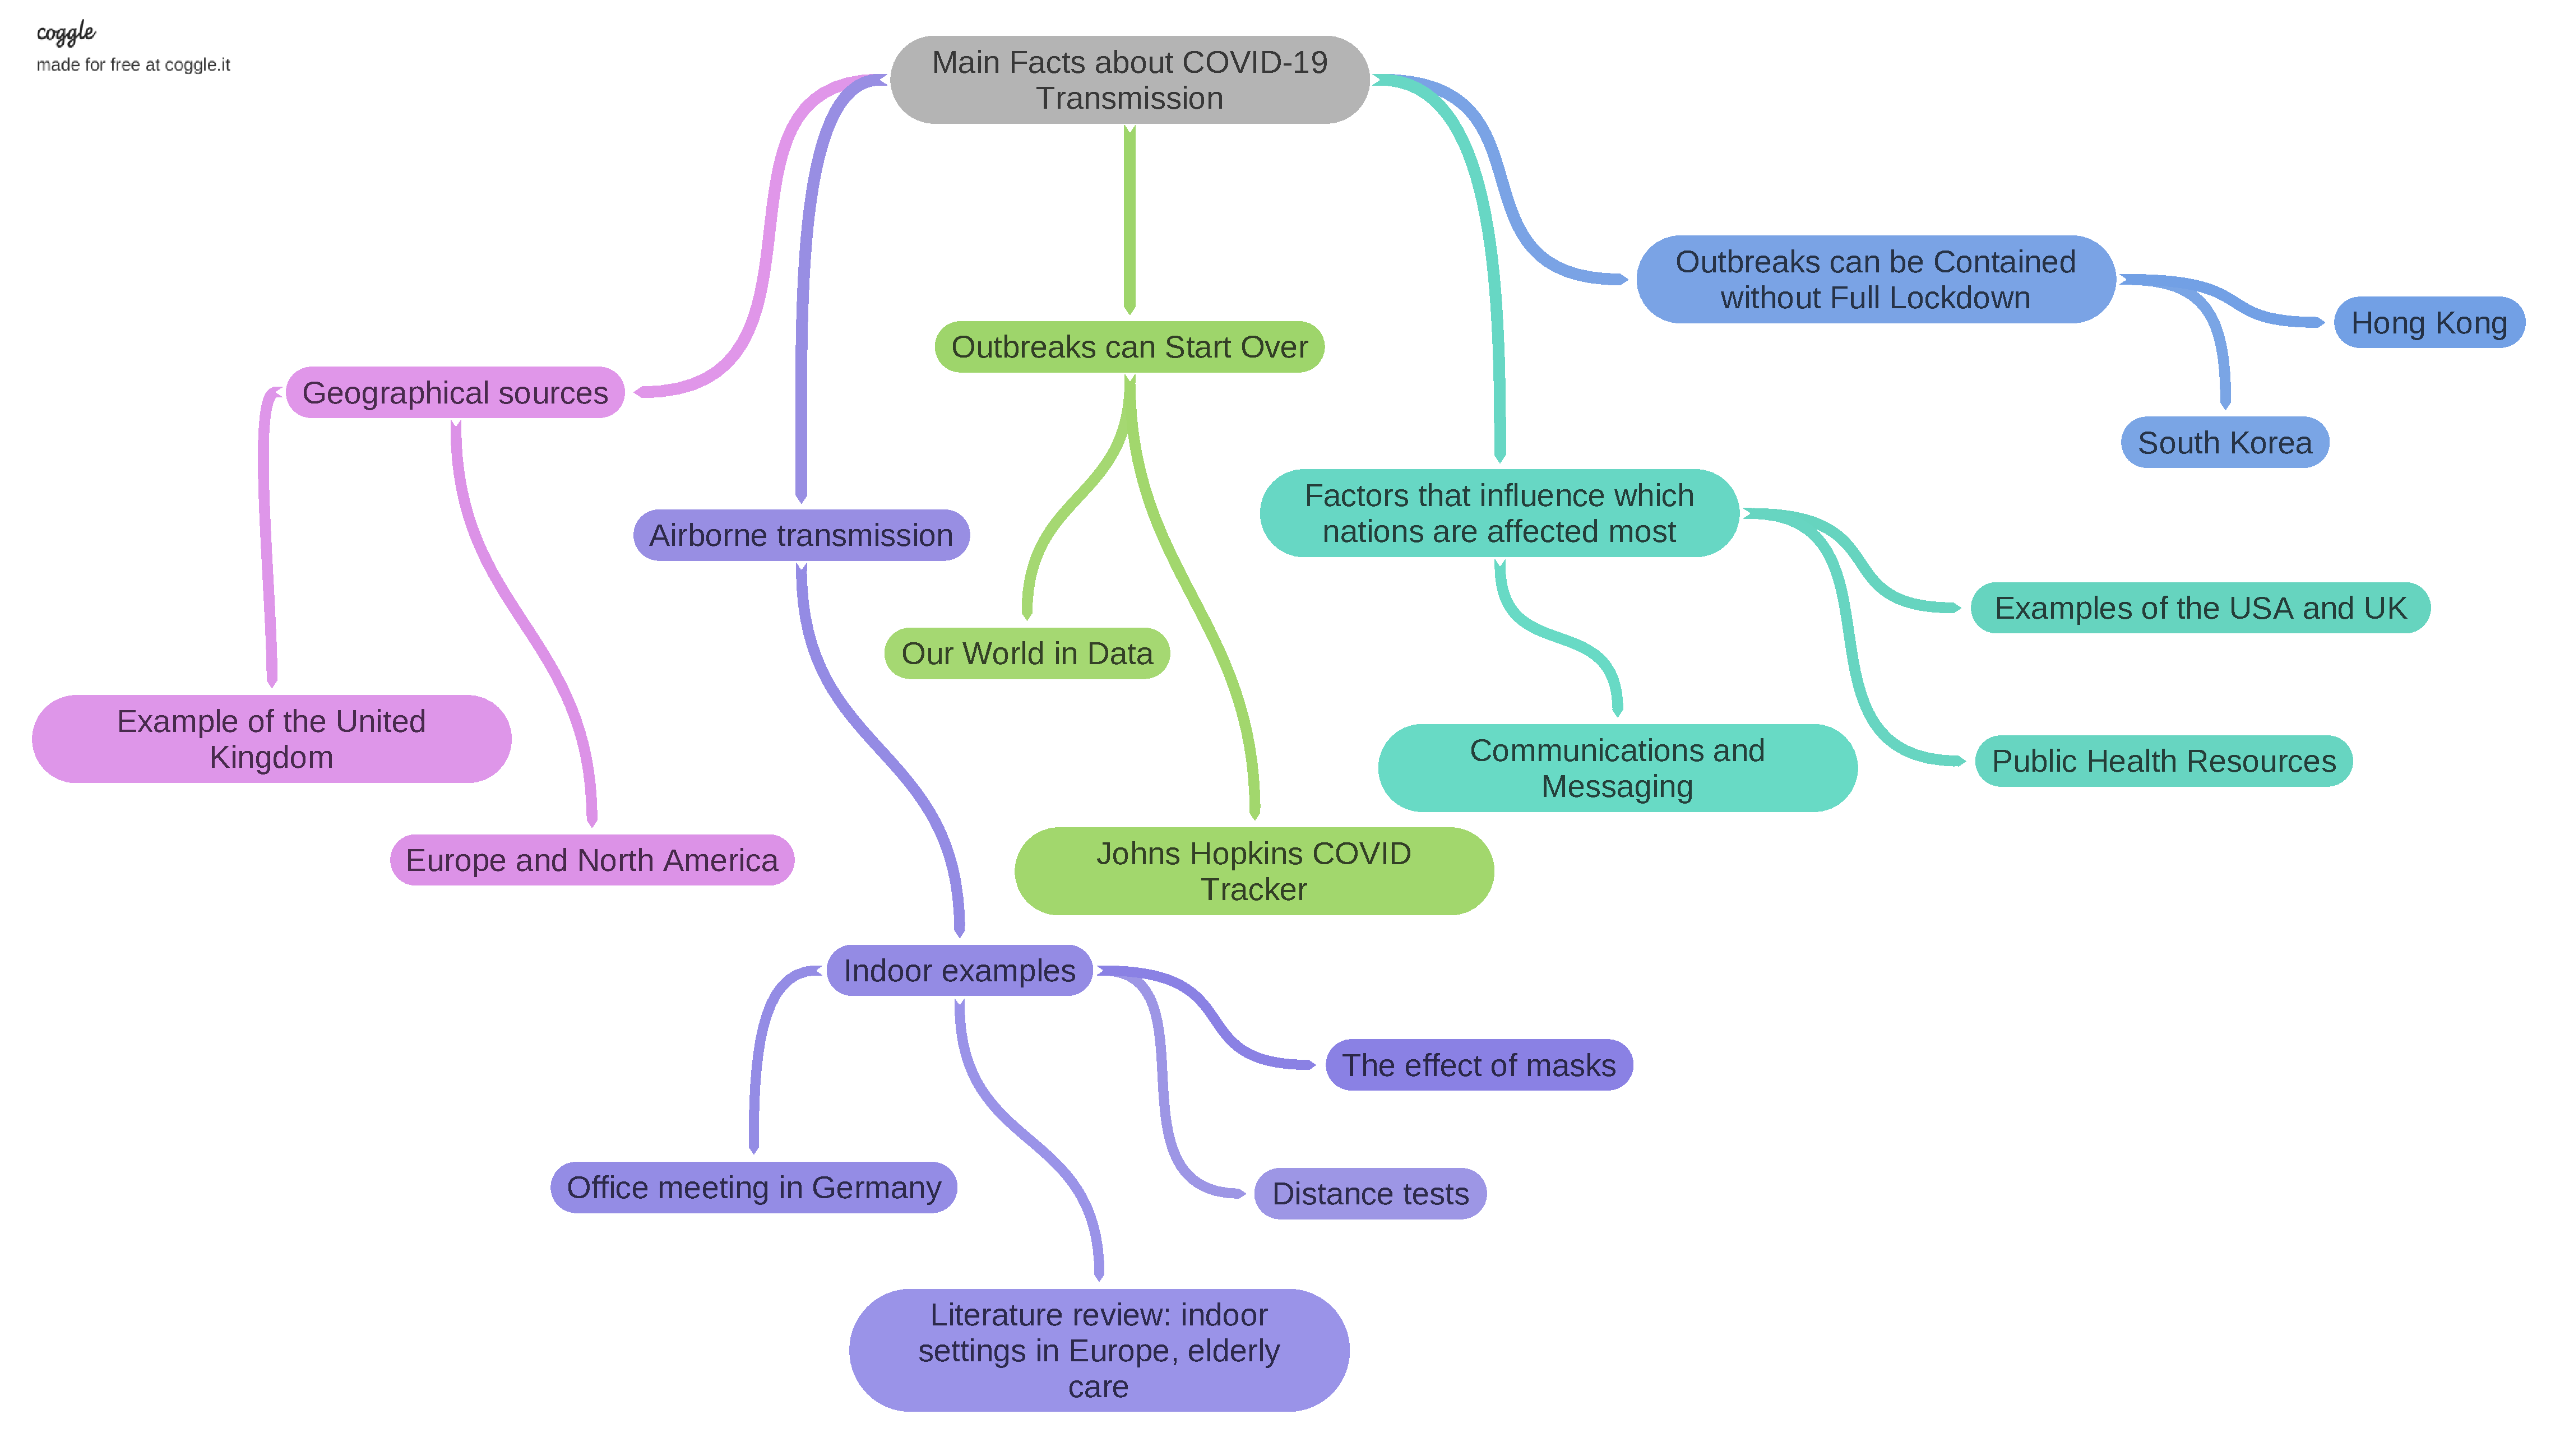
\includegraphics[width=0.95\textwidth]{figures/COVID_map.pdf}
\caption{\label{fig:covid1} This is an example of a mind map of the 5 things article.}
\end{figure}
\end{frame}

\begin{frame}{COVID-19 for a General Audience}
This could be a basic strategy in this extended example:
\begin{enumerate}
\item Start with the 5 things article
\item Branch off to the technical work
\begin{itemize}
\item What is research, and what is basic public health information
\item What is \textit{peer-reviewed} versus non-peer-reviewed work
\end{itemize}
\item Decide how much detail to keep from each branch
\item Interpret the graphs and the numbers: a few tips
\begin{itemize}
\item Never neglect the axes, always...\textbf{ALWAYS} define the axes for the reader
\item When describing shapes or curves or points on a chart, always use precise language
\item Avoid vague adjectives
\end{itemize}
\item Polish: use the delete button, use metaphor where appropriate, keep details in a hierarchy
\end{enumerate}
\end{frame}

\begin{frame}{COVID-19 for a General Audience}
\begin{figure}
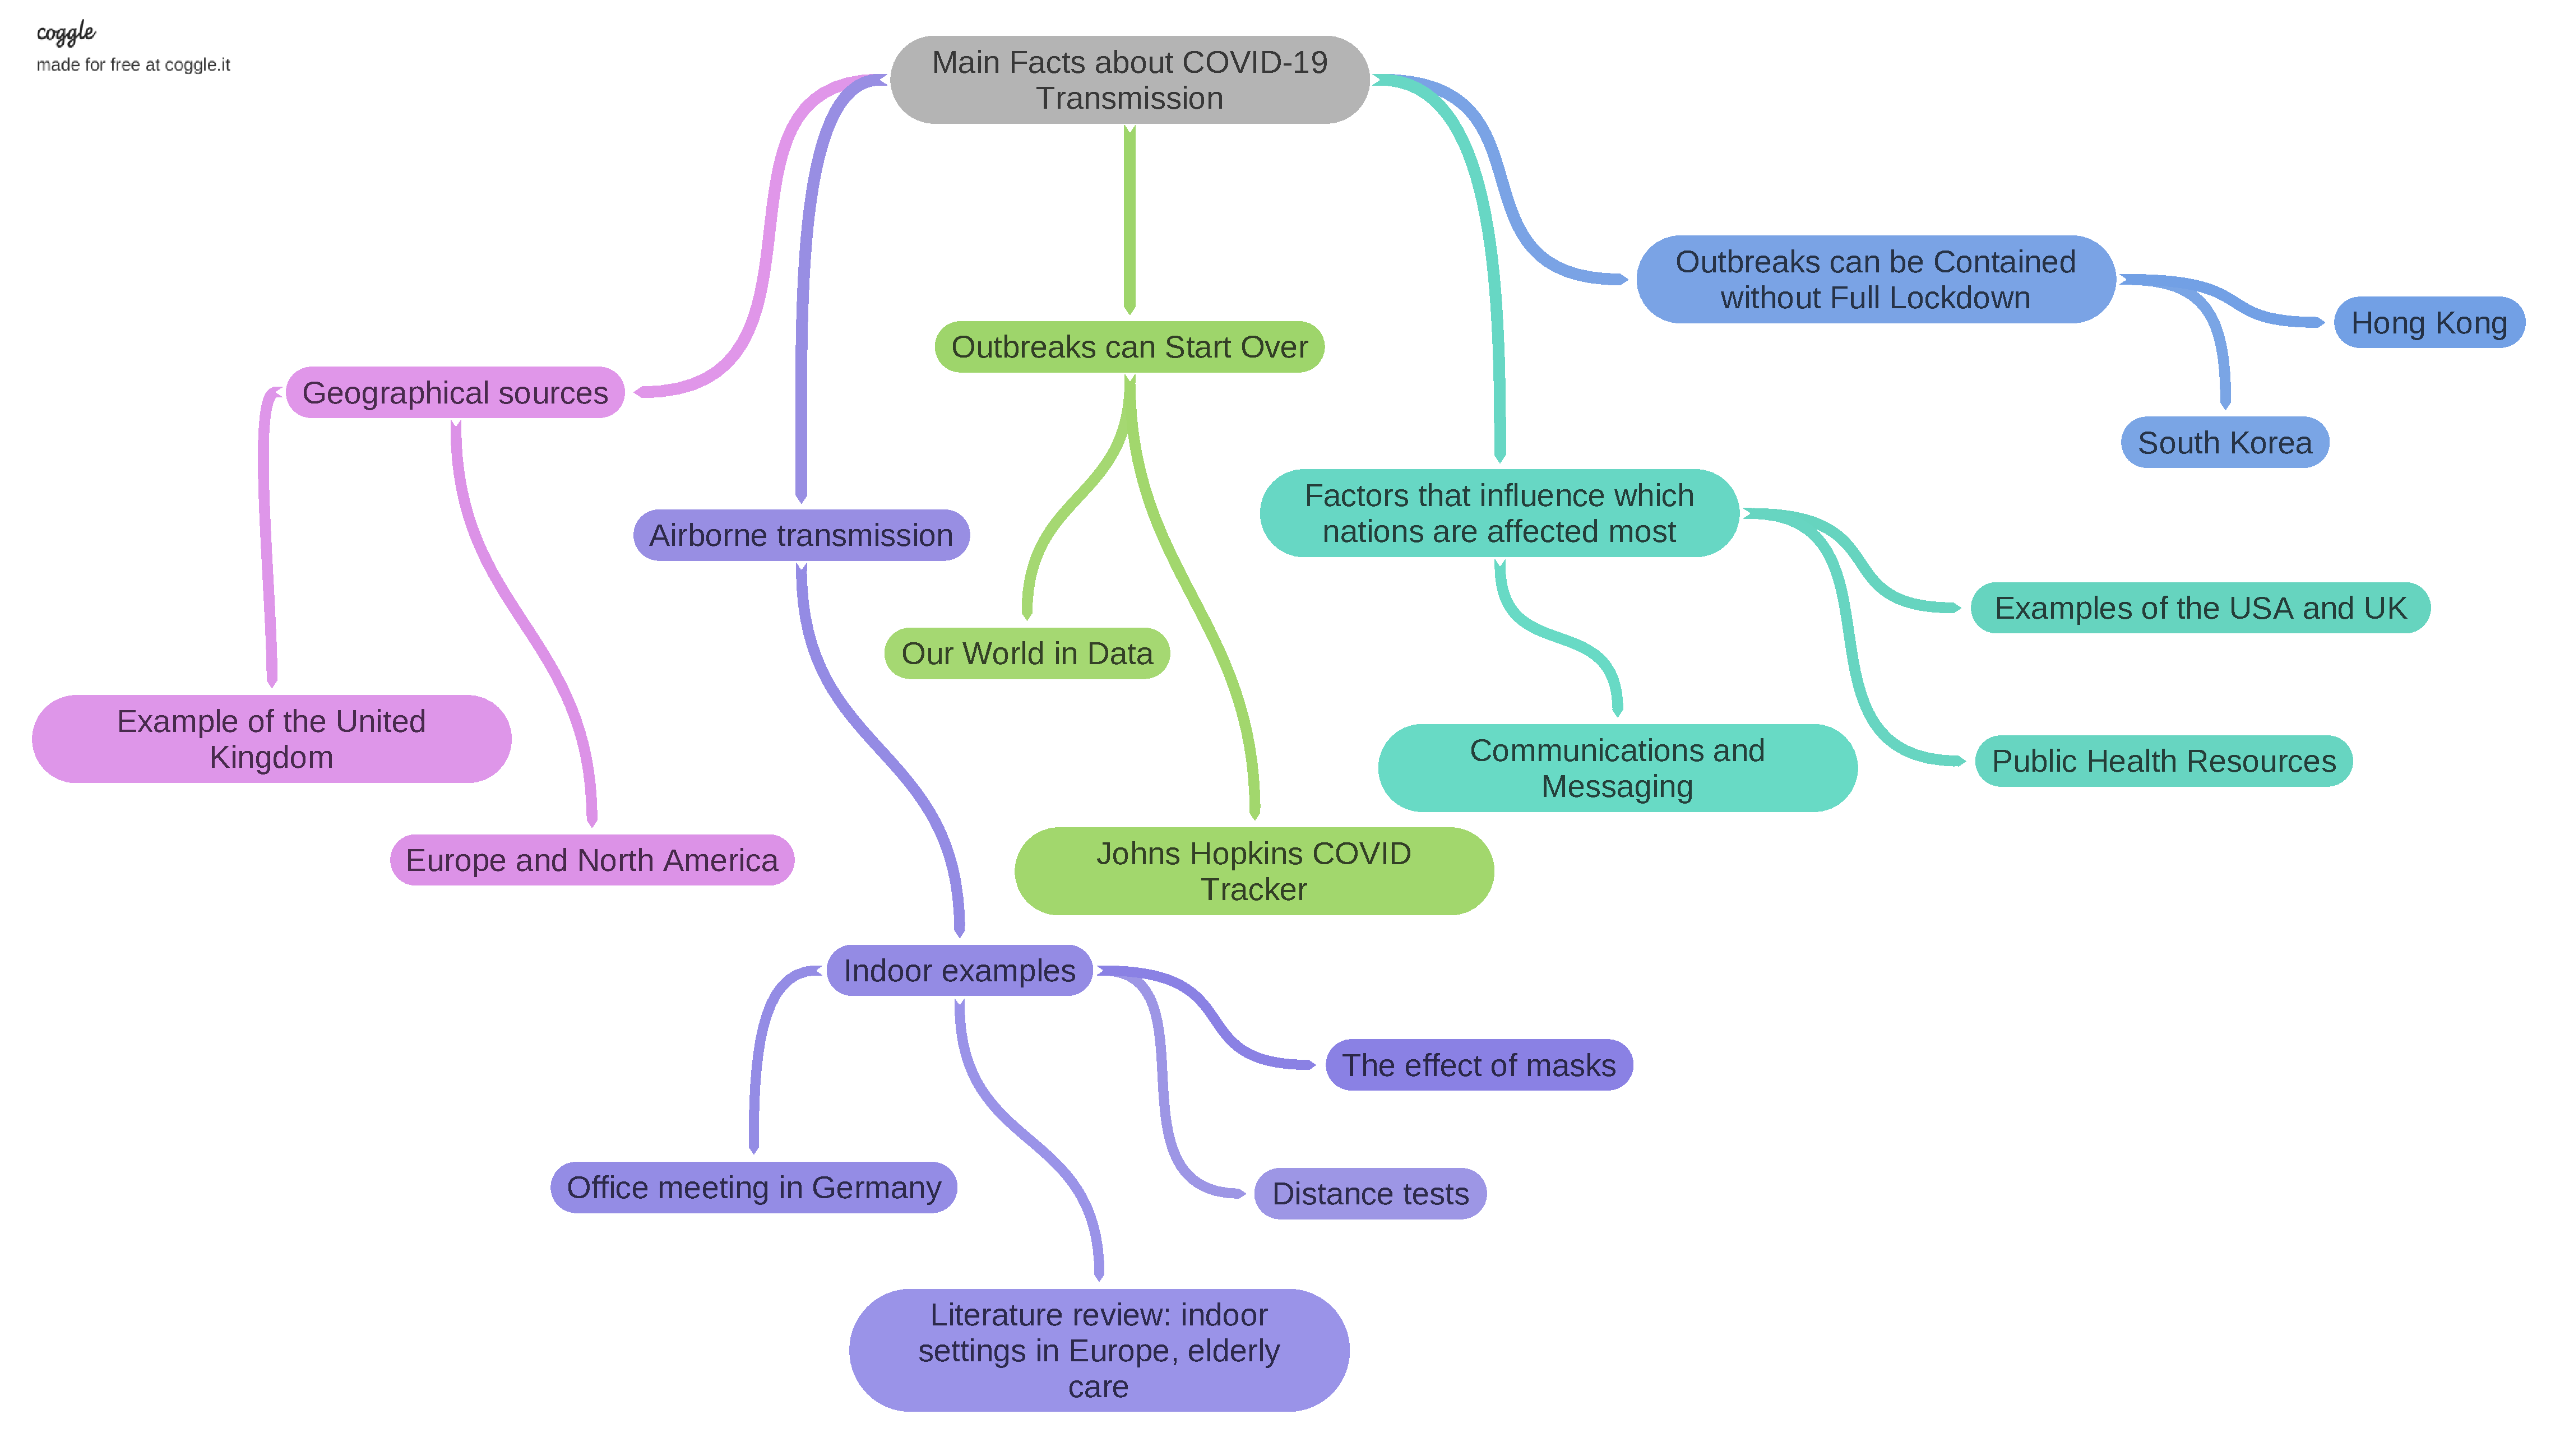
\includegraphics[width=0.95\textwidth]{figures/COVID_map.pdf}
\caption{\label{fig:covid2} This is an example of a mind map of the 5 things article.}
\end{figure}
\end{frame}

\begin{frame}{COVID-19 for a General Audience}
\textbf{Collaborate on Google Docs}: Go to Google Docs and log in with your Whittier College credentials.  Click on Shared with Me, and you should see the agenda page for today entitled Concise Writing, 2.  Using the Coggle map I've created, let's start writing!
\begin{enumerate}
\item Group A: Pink branch
\item Group B: Purple branch
\item Group C: Teal branch
\item Group D: Blue branch
\item Dr. Hanson: Lime branch
\end{enumerate}
Aaaaand...go!
\end{frame}

\section{Reviewing Leadership Essay Responses}

\begin{frame}{Reviewing Leadership Essay Responses}
\alert{Well done!} Several things stand out:
\begin{enumerate}
\item The organization is there.
\item The narrative or thread is kept intact (no digressions or tangents).
\item The writing mechanics need some work.
\item You will all be great Poets.
\end{enumerate}
\end{frame}

\begin{frame}{Reviewing Leadership Essay Responses}
\underline{Anonymous excerpt:}
\textit{At the time that I was an RA, I was also taking a piano lesson, doing a yoga class, and doing many hours of homework each night. I found that I had to think about multiple things at once most of the time in order to keep up with the expectations that were placed on me as a student leader. I often would forget about responsibilities as an RA, and on a few different occasions, I had to reschedule meetings with my dorm faculty because of my piano lessons, or because I had a test the next day that I could not spare the time to seperate myself from my studies.}
\end{frame}

\begin{frame}{Reviewing Leadership Essay Responses}
\textbf{How can we make this more concise?}
\textit{While serving as a residential assistant I was also taking piano and yoga lessons, and doing homework.  Multitasking was necessary to maintain my schedule and fulfill my responsibilities.  Focusing on homework, piano, and yoga occasionally subtracted from my focus on RA responsibilities.  For example, I had to reschedule meetings with my dorm faculty, or because I had a test the next day.}
\end{frame}

\begin{frame}{Reviewing Leadership Essay Responses}
\underline{Anonymous excerpt:}
\textit{The time spent in quarantine allowed me to work on my own time and think about
where my future was going; in a sense, “creating [my] own reality.” I’m pretty motivated to get
my work done, so I was able to hold higher confidence in myself and manage my time well. I
also tend to analyze things a lot, so i was able to look at the things i wanted to change about
myself and manage those barriers.}
\end{frame}

\begin{frame}{Reviewing Leadership Essay Responses}
\textbf{How can we make this more concise?}
\textit{The time spent in quarantine allowed me to work on my own and think about my future.  In a sense, I am “creating [my] own reality.”  With the solitude, motivation came easily and I confidently finished my work and managed time well.  I also set aside time to think about the things I wanted to change about myself.}
\end{frame}

\begin{frame}{Reviewing Leadership Essay Responses}
\small
\underline{Anonymous excerpt:}
\textit{In my community, La Puente, we are being raised into thinking we won't become
anything big but instead be someone mediocre. Students from xyz High School which I
attended have the mindset that they are going to just go through high school and see where life
takes you. Sports for instants isn't taken all serious because nobody has ever continued playing
sports at a college level or they just think of it as a joke. What about those kids that have a dream
and want to play at the next level and have the passion for the sport. Many of those students
transfer out to a “better” school to get notice from colleges. Well I was one of those kids that
wanted to play college ball. Start of my freshman year probably the weakest and smallest kid on
the field that nobody thought would be good. Lots of people made fun of me because I told
myself that one day imma play college ball. Many of the seniors of the football team said
“You're too small”, “No college gonna see you”. At one point I actually listened to them and
almost quit because I was very gullible and believed in almost anything.}
\end{frame}

\begin{frame}{Reviewing Leadership Essay Responses}
\textbf{How can we make this more concise?}
\textit{La Puente is a community in which young men are raised to believe they will not achieve much in
their lives after high school. At my high school, xyz High School, sports are not taken
seriously because few go on to play in college. I was one student who desired to play at the next
level in college, despite being smaller and weaker in my freshman year. I told my teammates I
wanted to play in college but they mocked me, saying that I was too small or that college
recruiters were not going to notice me. I came close to quitting after hearing this type of remark,
almost beginning to believe them.}
\end{frame}

\begin{frame}{Reviewing Leadership Essay Responses}
\underline{Anonymous excerpt:}
\textit{Now i absolutely love my team and loved getting to be their captain but i spent a
decent amount of time on my own and talking to my co captain trying to figure out the best way
to lead a group of teenagers who don't really want to listen to another teenager tell them what to
do, and it was difficult. Building the bond of not only being a friend but someone with authority
was hard, we could have fun but at the end of the day i still had to be respected. When the
author writes about coming up with ideas and how the first thought is never his own, I feel like
that is how I feel when trying to resolve things. It's always `` how would xyz do this'' instead of
me figuring out the best way to handle something...}
\end{frame}

\begin{frame}{Reviewing Leadership Essay Responses}
\textbf{How can we make this more concise?}
\textit{I love my team and being their captain was a privilege.  I spent time thinking alone and talking to my co-captain about how to lead teenagers who do not listen.  We felt it necessary to build the bond of friendship with the team, but maintain the authority necessary for quality results in competition.  This was difficult.  When the author writes about creating plans, he remarks that the first idea is not the best idea and is often attributed to someone elsed.  When trying to resolve team issues, I would ask myself how another person would solve it.  The best approach seems to be determining the answer on my own.}
\end{frame}

\section{General Audiences need Fewer Words}

\begin{frame}{Pro-tips for your group Projects}
Let's watch the TED talk on the first picture of a black hole: \\ \vspace{0.5cm}
\url{https://www.ted.com/talks/katie_bouman_how_to_take_a_picture_of_a_black_hole?utm_campaign=tedspread&utm_medium=referral&utm_source=tedcomshare}
\end{frame}

\begin{frame}{Pro-tips for your group Projects}
\textbf{\alert{What stood out to you?}}
\begin{enumerate}
\item Did you hear any metaphors or analogies?
\item Were any equations replaced with graphics?
\item Did you hear why radio frequencies are the important wavelength (as opposed to optical light)?
\item Did you understand how we built a telescope the size of the Earth?
\end{enumerate}
\end{frame}

\section{Conclusion}

\begin{frame}{Summary}
\textbf{Week 2}: \textit{Concise writing II:} In Week 2, we will focus on reading a piece of science writing, and creating your \textit{own} writing that tailors the story to a particular audience.
\begin{itemize}
\item Exercises: work in teams to produce a piece of science writing intended for a broad audience that weaves together information from a variety of sources: (a) a TED talk (b) a scientific journal article (c) and resources like Wikipedia and Google Scholar
\item Homework: writing a post designed for social media about a piece of science that grabs the attention of a wide audience, and attempts to convince that audience that the science is interesting
\item Exploration topic: Black hole observations
\end{itemize}
\end{frame}

\bibliographystyle{plain}
\section{Bibliography}

\bibliography{bibfile}

\end{document}
